\begin{figure}[htp]
  \centering
  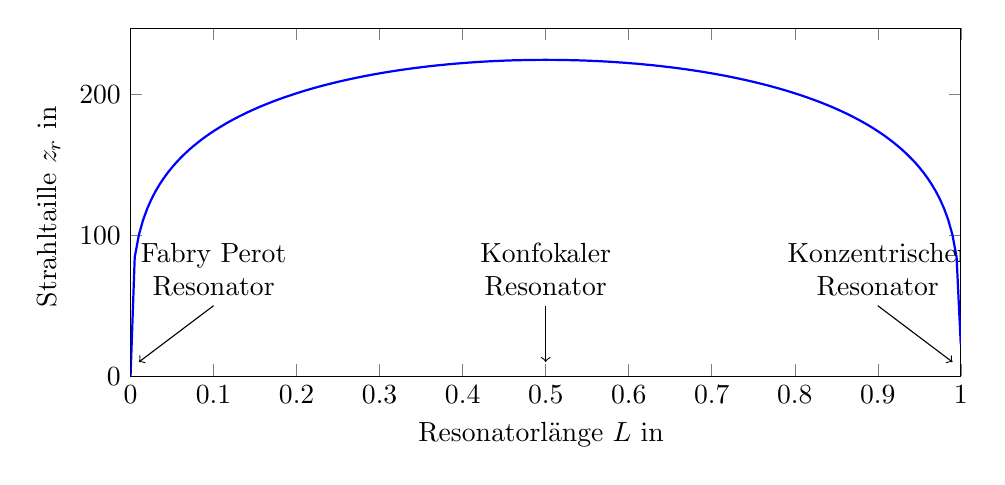
\begin{tikzpicture}[every text node part/.style={align=center}]
    \begin{axis}[disabledatascaling, width=\textwidth, height=6cm, ylabel=Strahltaille $z_r$ in \si{\micro\metre}, xlabel=Resonatorlänge $L$ in \si{\metre}, xmin=0, xmax=1, ymin = 0, samples = 200, domain=0:1]
      \addplot[blue, thick] {(2*0.5*x-x^2)^(1/4)*(0.6328/(2*pi))^(1/2)*1000};
      \draw[<-] (.5,10) -- (.5,50)node[above]{Konfokaler\\ Resonator};
      \draw[<-] (.01,10) -- (.1,50)node[above]{Fabry Perot\\ Resonator};
      \draw[<-] (.99,10) -- (.9,50)node[above]{Konzentrischer\\ Resonator};
    \end{axis}
\end{tikzpicture}
  \caption{Radius der Strahltaille $z_r$ als Funktion der Resonatorlänge $L$ eines symmetrischen Resonators mit Krümmungsradius $R=\SI{0.5}{\metre}$ der Spiegel.}
  \label{fig:Strahltaille_Theorie}
\end{figure}
